\subsection{part a}
\begin{itemize}
    \item $K=0.5$
    \begin{figure}[H]
        \caption{Nichols chart for $KG, (K=0.5)$}
        \centering
        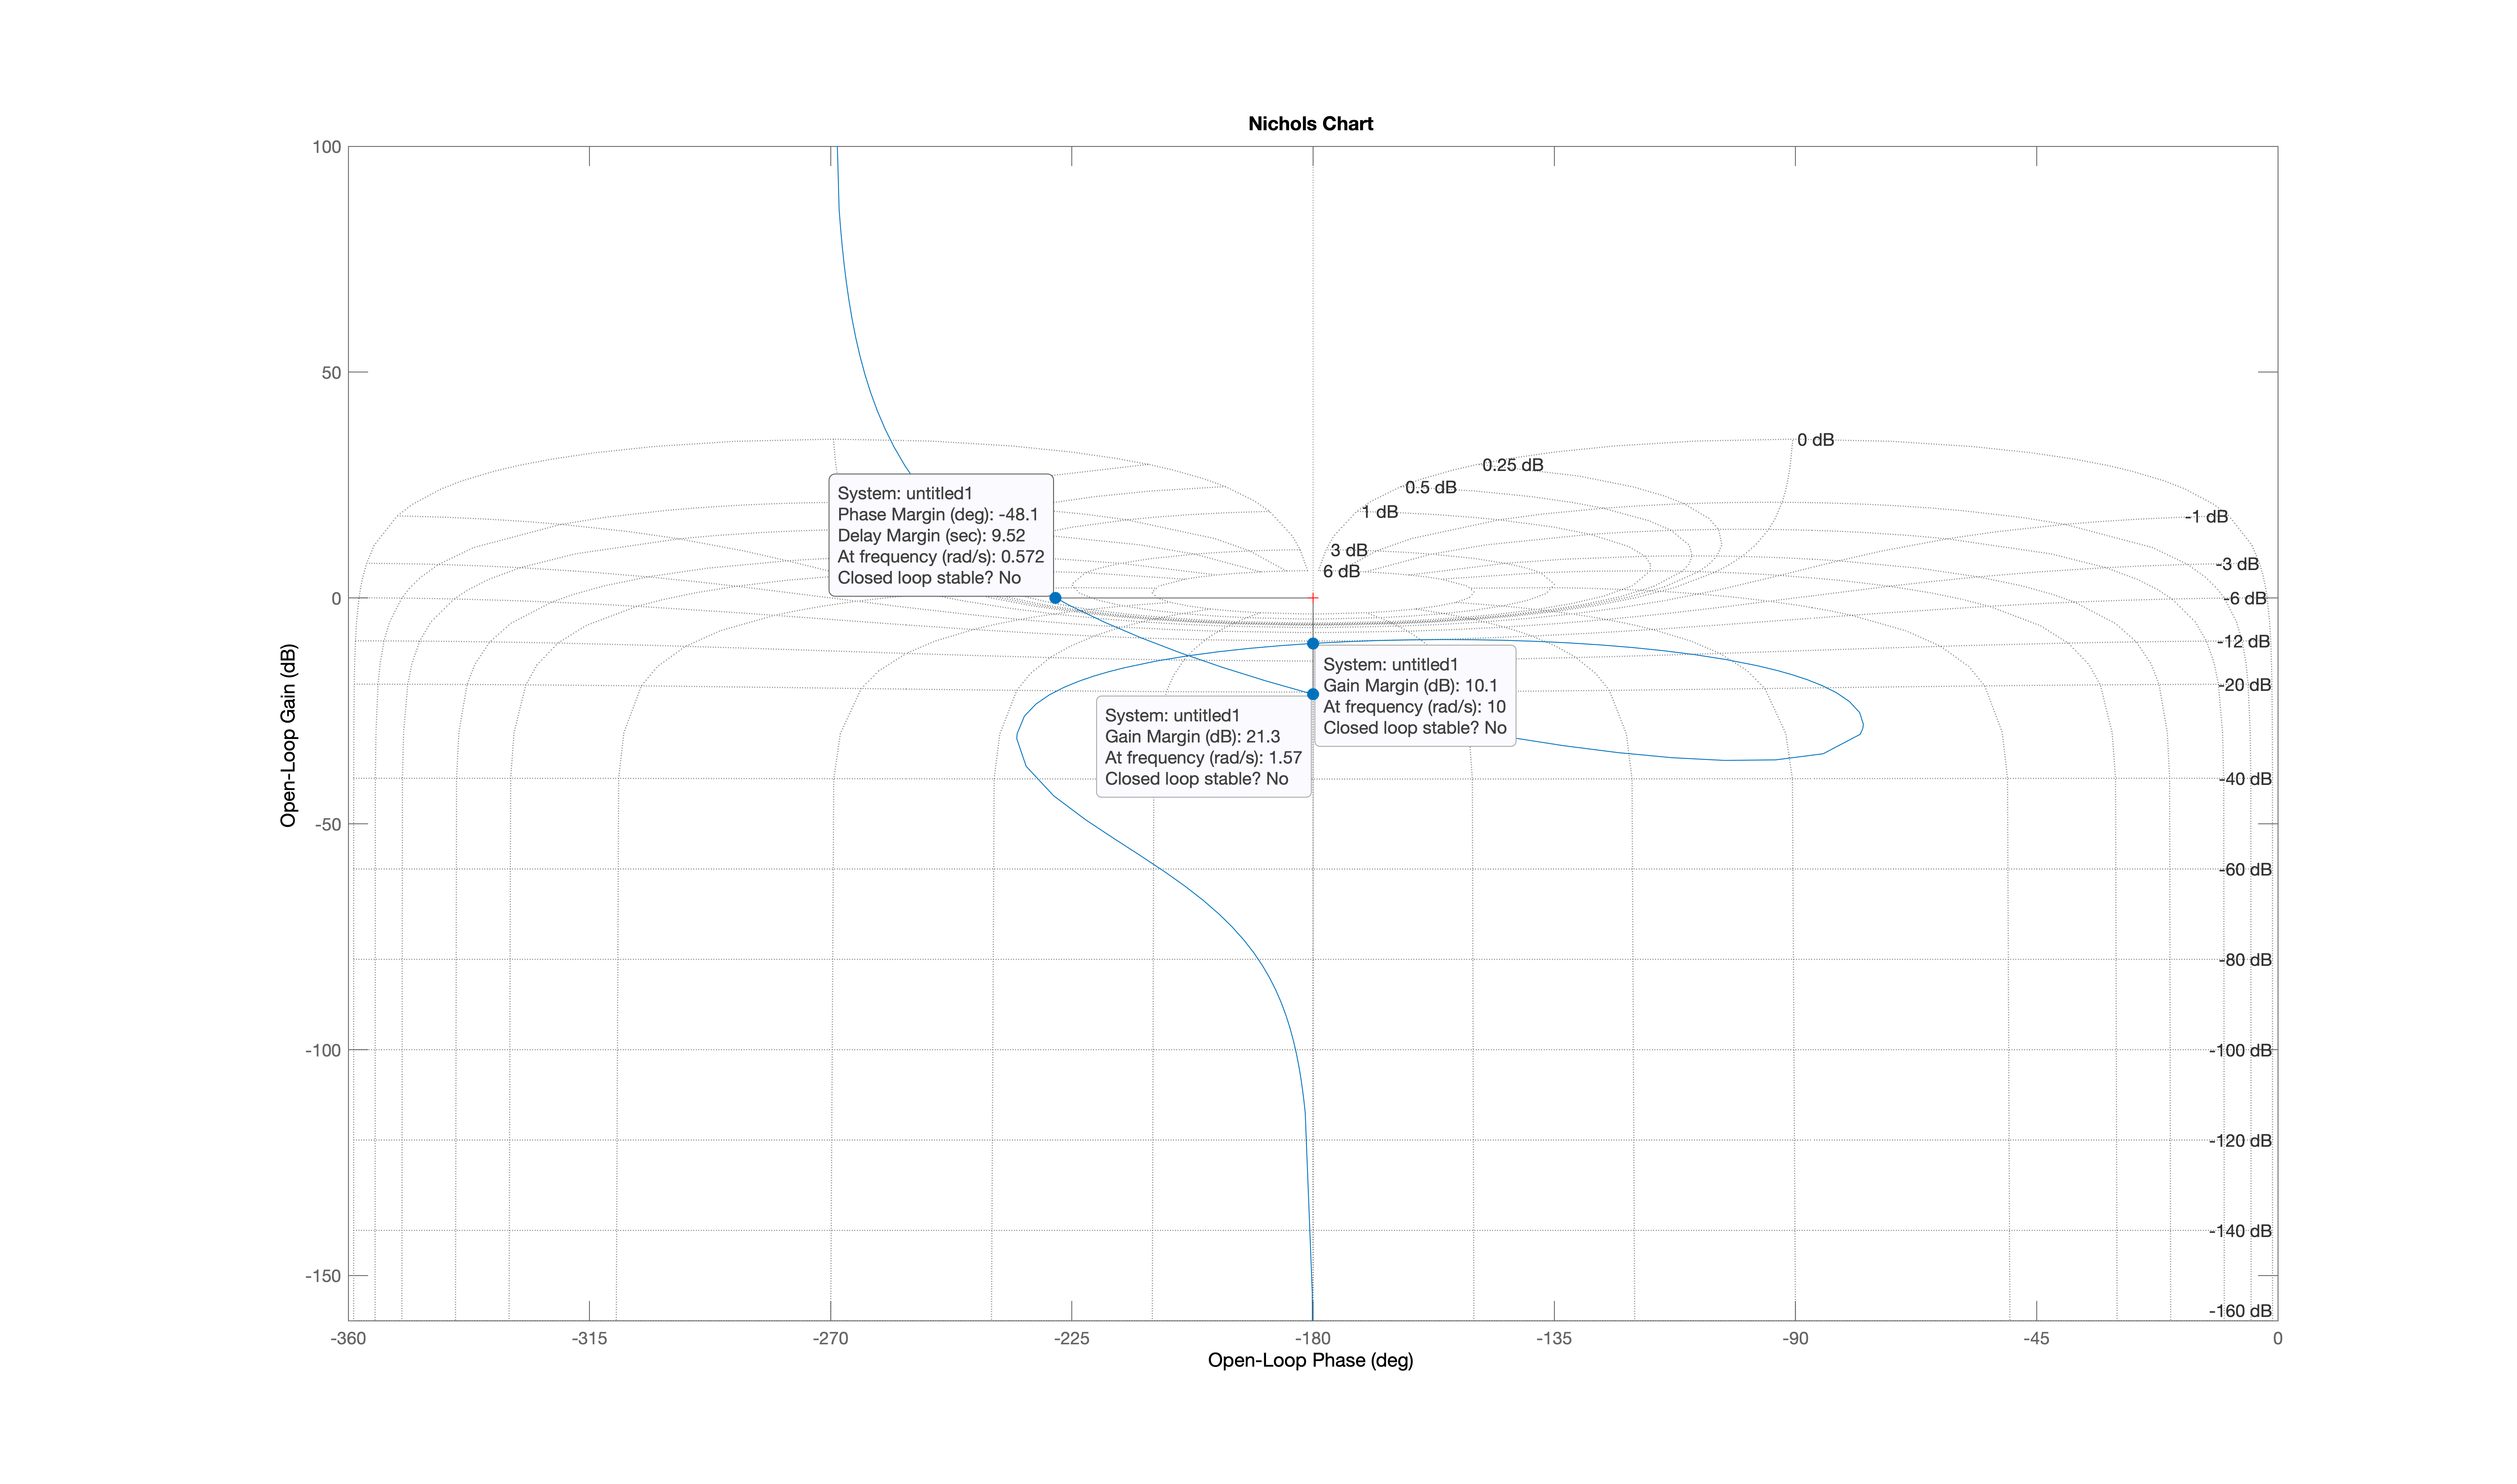
\includegraphics[width=16cm]{../Figure/Q1/Q1_a/Q1_aK_0.5.png}
    \end{figure}
    \item $K=1$
    \begin{figure}[H]
        \caption{Nichols chart for $KG, (K=1)$}
        \centering
        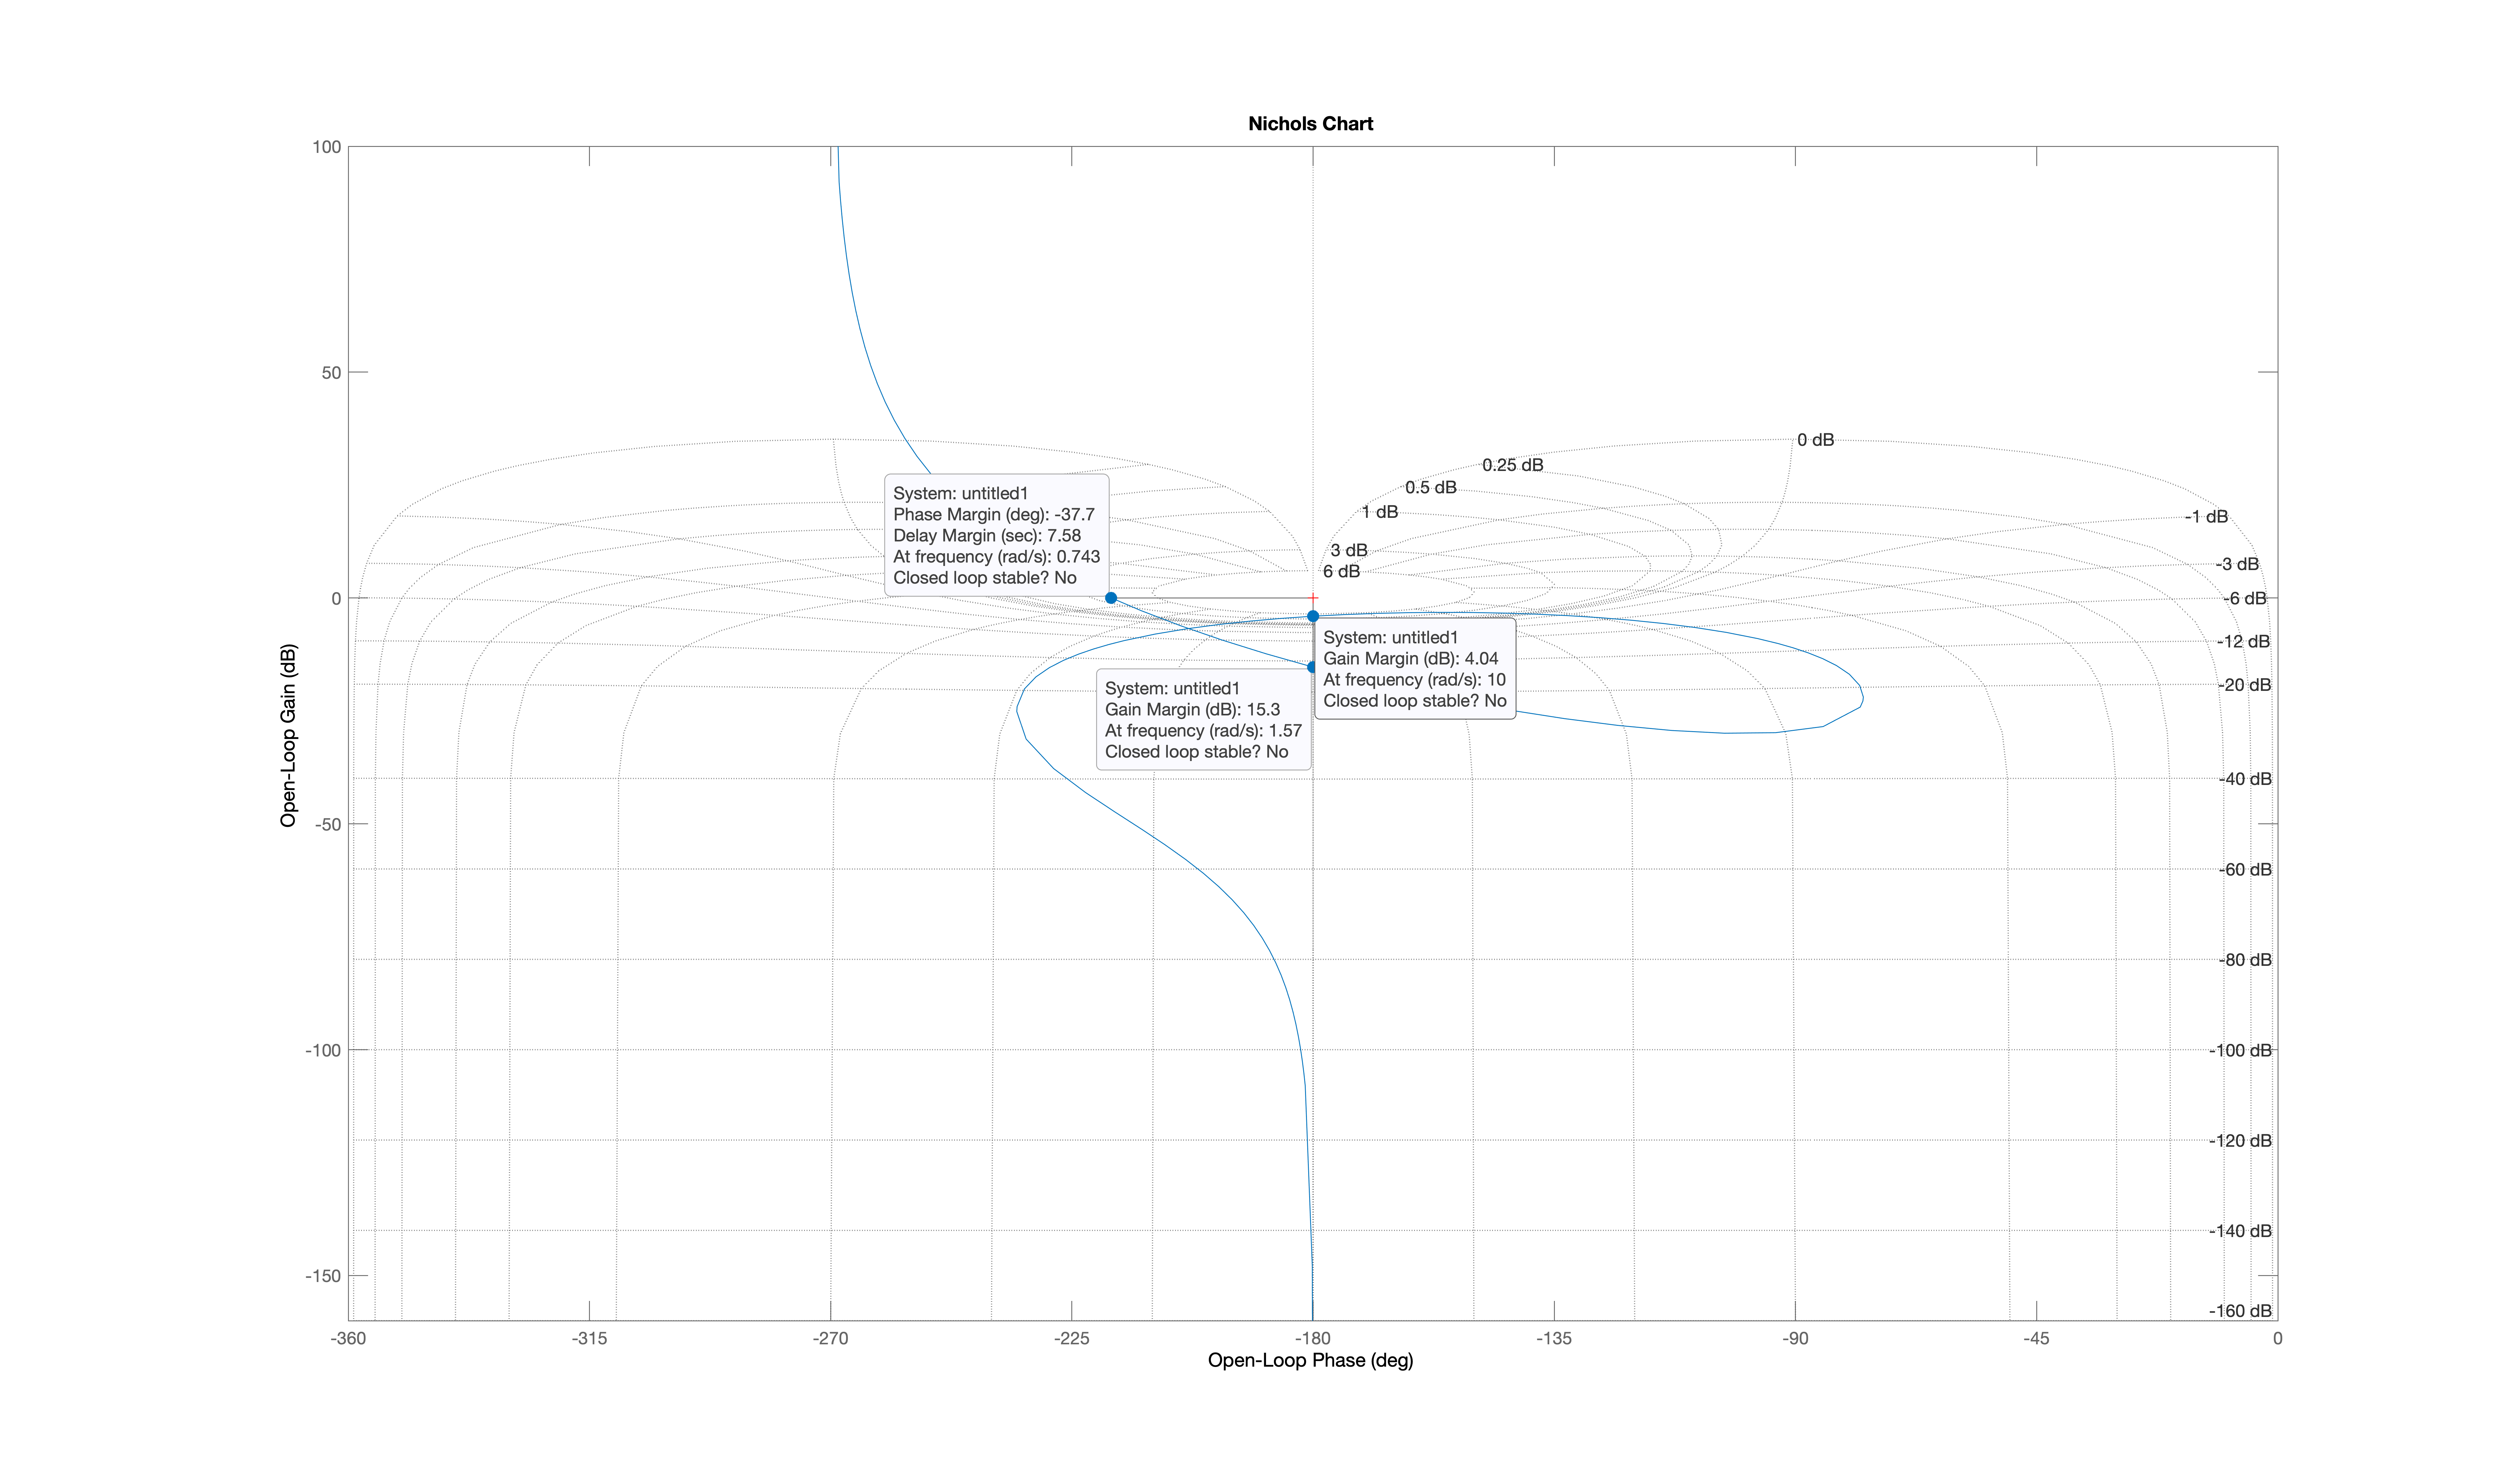
\includegraphics[width=16cm]{../Figure/Q1/Q1_a/Q1_aK_1.png}
    \end{figure}
    \item $K=5$
    \begin{figure}[H]
        \caption{Nichols chart for $KG, (K=5)$}
        \centering
        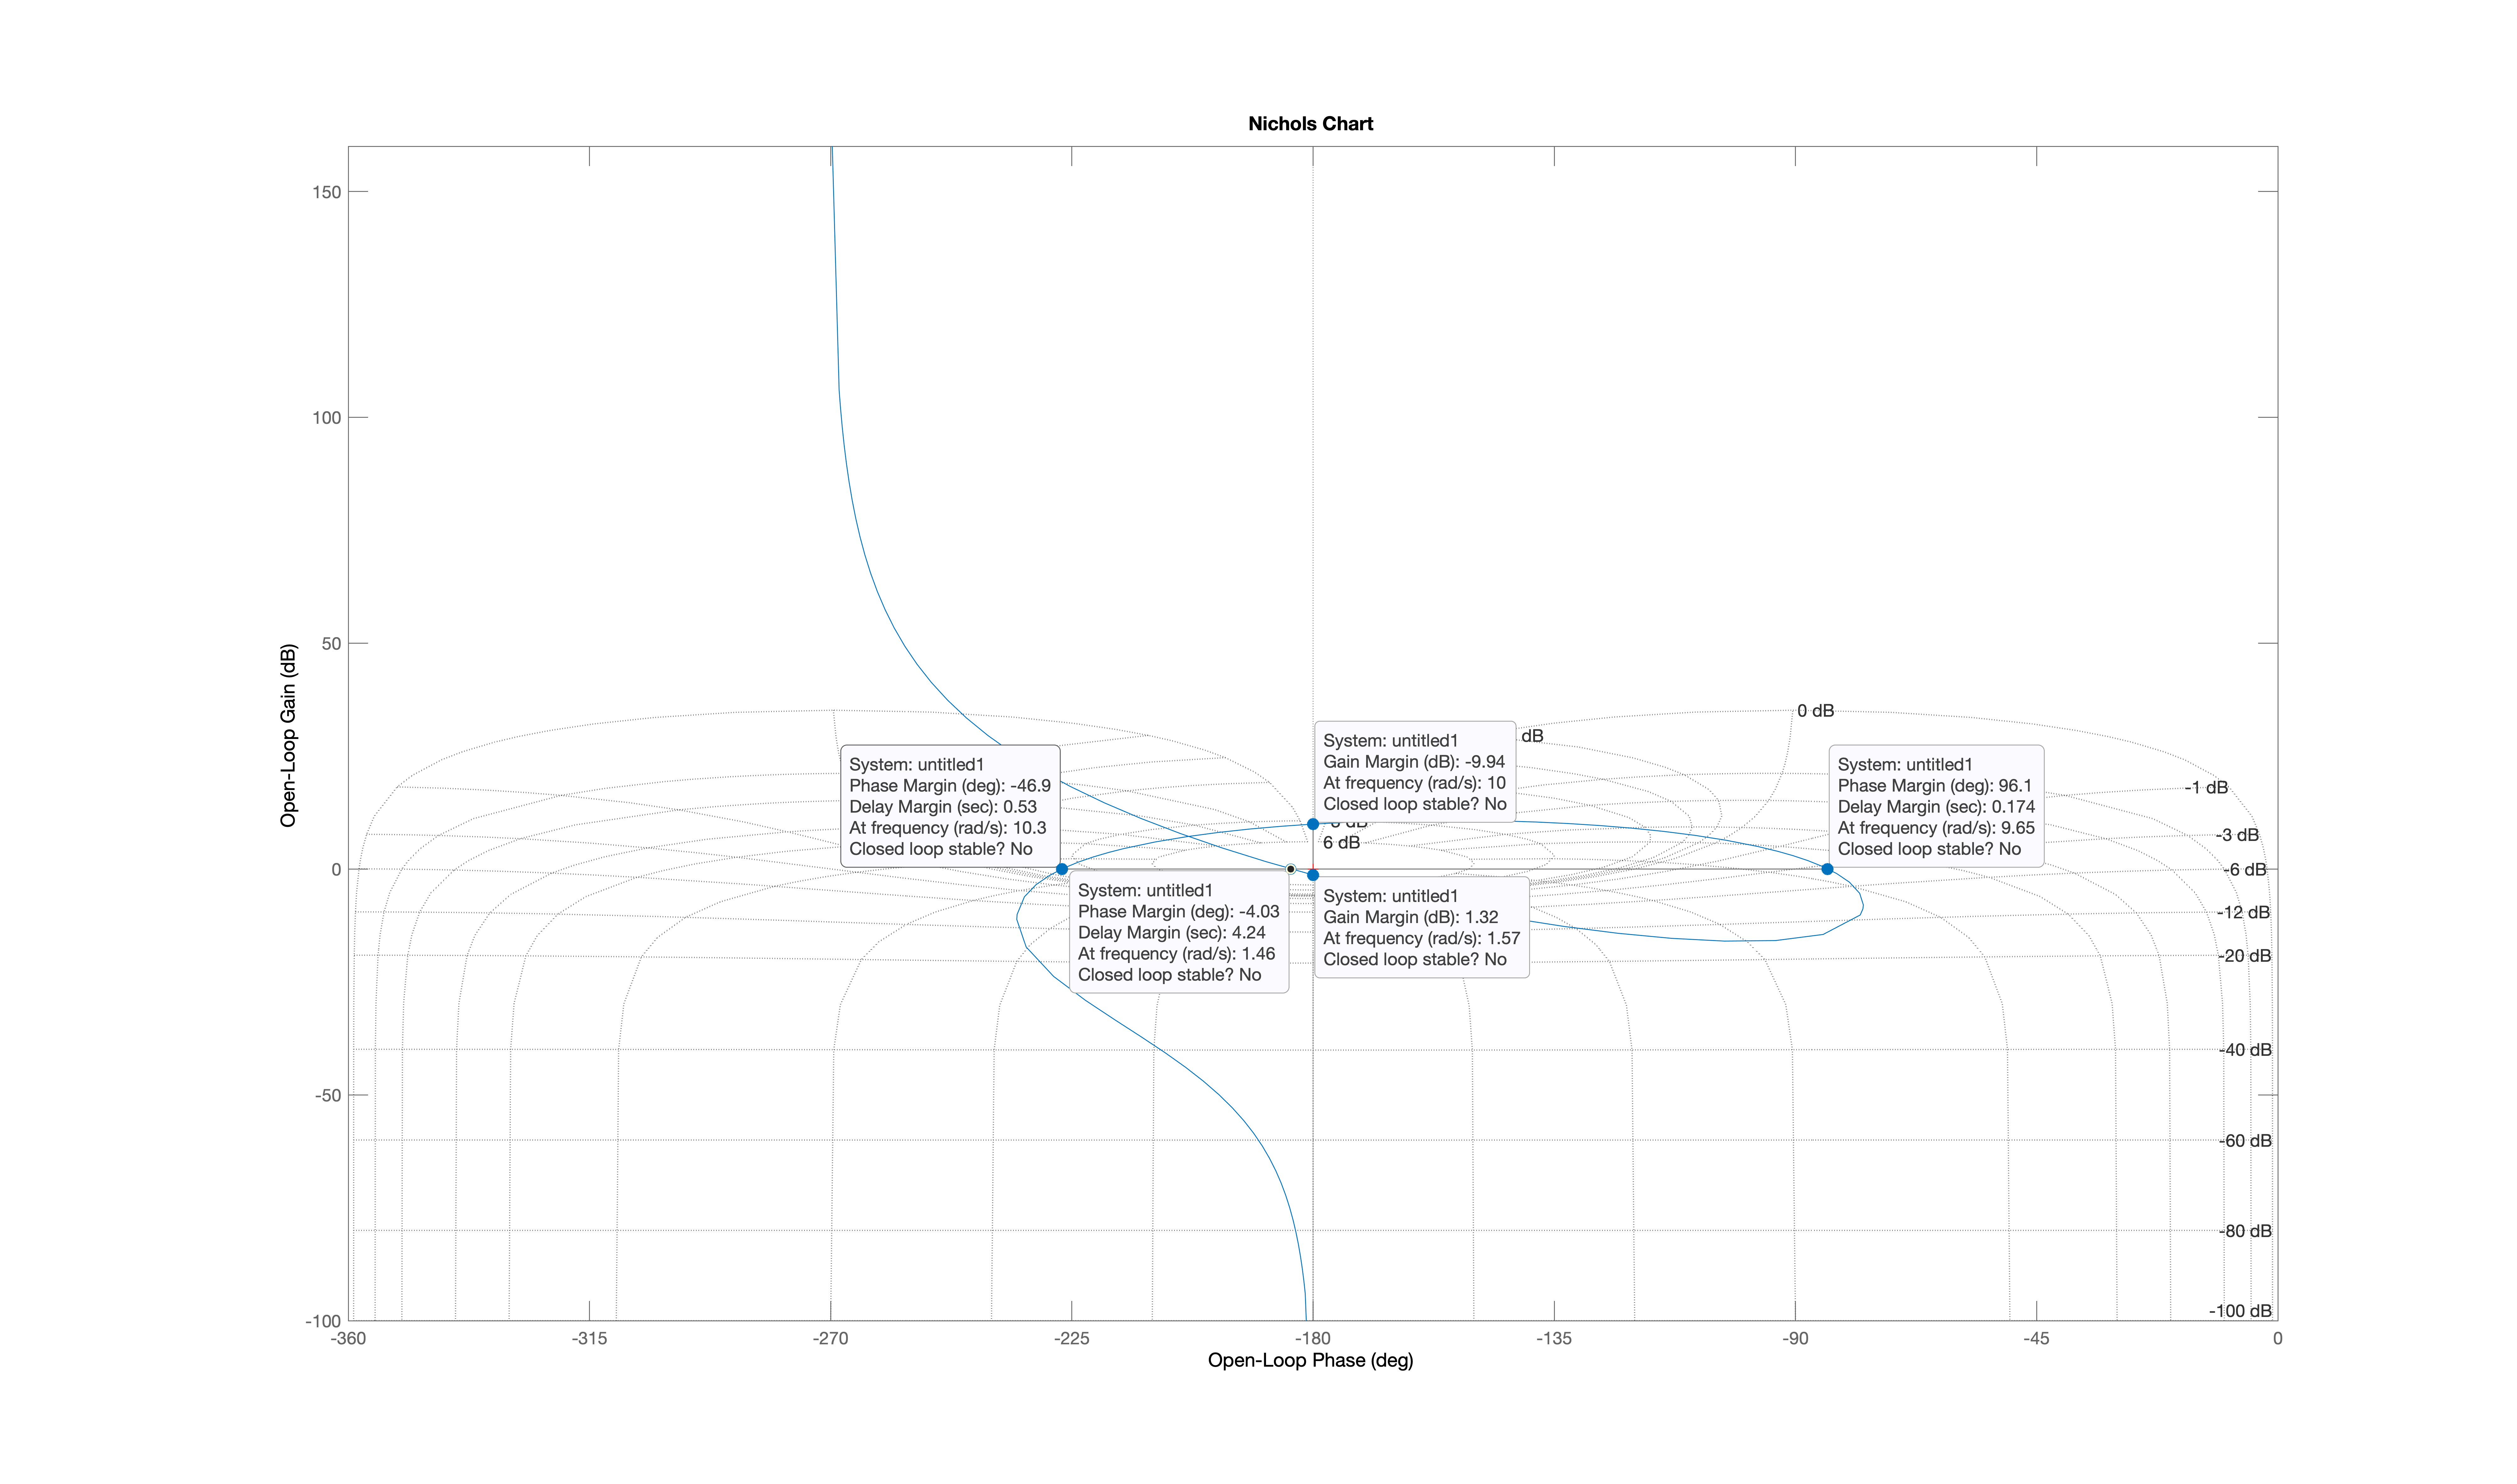
\includegraphics[width=16cm]{../Figure/Q1/Q1_a/Q1_aK_5.png}
    \end{figure}
\end{itemize}
Phase margin and gain margin are shown in above figures and all closed loop systems are unstable with $K$ form 1 to 5. In all of them phase margin is negetive.